\documentclass[]{article}
\usepackage{lmodern}
\usepackage{amssymb,amsmath}
\usepackage{ifxetex,ifluatex}
\usepackage{fixltx2e} % provides \textsubscript
\ifnum 0\ifxetex 1\fi\ifluatex 1\fi=0 % if pdftex
  \usepackage[T1]{fontenc}
  \usepackage[utf8]{inputenc}
\else % if luatex or xelatex
  \ifxetex
    \usepackage{mathspec}
  \else
    \usepackage{fontspec}
  \fi
  \defaultfontfeatures{Ligatures=TeX,Scale=MatchLowercase}
\fi
% use upquote if available, for straight quotes in verbatim environments
\IfFileExists{upquote.sty}{\usepackage{upquote}}{}
% use microtype if available
\IfFileExists{microtype.sty}{%
\usepackage[]{microtype}
\UseMicrotypeSet[protrusion]{basicmath} % disable protrusion for tt fonts
}{}
\PassOptionsToPackage{hyphens}{url} % url is loaded by hyperref
\usepackage[unicode=true]{hyperref}
\hypersetup{
            pdftitle={Assignment 3: Data Exploration},
            pdfauthor={Emily McNamara},
            pdfborder={0 0 0},
            breaklinks=true}
\urlstyle{same}  % don't use monospace font for urls
\usepackage[margin=2.00cm]{geometry}
\usepackage{color}
\usepackage{fancyvrb}
\newcommand{\VerbBar}{|}
\newcommand{\VERB}{\Verb[commandchars=\\\{\}]}
\DefineVerbatimEnvironment{Highlighting}{Verbatim}{commandchars=\\\{\}}
% Add ',fontsize=\small' for more characters per line
\usepackage{framed}
\definecolor{shadecolor}{RGB}{248,248,248}
\newenvironment{Shaded}{\begin{snugshade}}{\end{snugshade}}
\newcommand{\KeywordTok}[1]{\textcolor[rgb]{0.13,0.29,0.53}{\textbf{#1}}}
\newcommand{\DataTypeTok}[1]{\textcolor[rgb]{0.13,0.29,0.53}{#1}}
\newcommand{\DecValTok}[1]{\textcolor[rgb]{0.00,0.00,0.81}{#1}}
\newcommand{\BaseNTok}[1]{\textcolor[rgb]{0.00,0.00,0.81}{#1}}
\newcommand{\FloatTok}[1]{\textcolor[rgb]{0.00,0.00,0.81}{#1}}
\newcommand{\ConstantTok}[1]{\textcolor[rgb]{0.00,0.00,0.00}{#1}}
\newcommand{\CharTok}[1]{\textcolor[rgb]{0.31,0.60,0.02}{#1}}
\newcommand{\SpecialCharTok}[1]{\textcolor[rgb]{0.00,0.00,0.00}{#1}}
\newcommand{\StringTok}[1]{\textcolor[rgb]{0.31,0.60,0.02}{#1}}
\newcommand{\VerbatimStringTok}[1]{\textcolor[rgb]{0.31,0.60,0.02}{#1}}
\newcommand{\SpecialStringTok}[1]{\textcolor[rgb]{0.31,0.60,0.02}{#1}}
\newcommand{\ImportTok}[1]{#1}
\newcommand{\CommentTok}[1]{\textcolor[rgb]{0.56,0.35,0.01}{\textit{#1}}}
\newcommand{\DocumentationTok}[1]{\textcolor[rgb]{0.56,0.35,0.01}{\textbf{\textit{#1}}}}
\newcommand{\AnnotationTok}[1]{\textcolor[rgb]{0.56,0.35,0.01}{\textbf{\textit{#1}}}}
\newcommand{\CommentVarTok}[1]{\textcolor[rgb]{0.56,0.35,0.01}{\textbf{\textit{#1}}}}
\newcommand{\OtherTok}[1]{\textcolor[rgb]{0.56,0.35,0.01}{#1}}
\newcommand{\FunctionTok}[1]{\textcolor[rgb]{0.00,0.00,0.00}{#1}}
\newcommand{\VariableTok}[1]{\textcolor[rgb]{0.00,0.00,0.00}{#1}}
\newcommand{\ControlFlowTok}[1]{\textcolor[rgb]{0.13,0.29,0.53}{\textbf{#1}}}
\newcommand{\OperatorTok}[1]{\textcolor[rgb]{0.81,0.36,0.00}{\textbf{#1}}}
\newcommand{\BuiltInTok}[1]{#1}
\newcommand{\ExtensionTok}[1]{#1}
\newcommand{\PreprocessorTok}[1]{\textcolor[rgb]{0.56,0.35,0.01}{\textit{#1}}}
\newcommand{\AttributeTok}[1]{\textcolor[rgb]{0.77,0.63,0.00}{#1}}
\newcommand{\RegionMarkerTok}[1]{#1}
\newcommand{\InformationTok}[1]{\textcolor[rgb]{0.56,0.35,0.01}{\textbf{\textit{#1}}}}
\newcommand{\WarningTok}[1]{\textcolor[rgb]{0.56,0.35,0.01}{\textbf{\textit{#1}}}}
\newcommand{\AlertTok}[1]{\textcolor[rgb]{0.94,0.16,0.16}{#1}}
\newcommand{\ErrorTok}[1]{\textcolor[rgb]{0.64,0.00,0.00}{\textbf{#1}}}
\newcommand{\NormalTok}[1]{#1}
\usepackage{graphicx,grffile}
\makeatletter
\def\maxwidth{\ifdim\Gin@nat@width>\linewidth\linewidth\else\Gin@nat@width\fi}
\def\maxheight{\ifdim\Gin@nat@height>\textheight\textheight\else\Gin@nat@height\fi}
\makeatother
% Scale images if necessary, so that they will not overflow the page
% margins by default, and it is still possible to overwrite the defaults
% using explicit options in \includegraphics[width, height, ...]{}
\setkeys{Gin}{width=\maxwidth,height=\maxheight,keepaspectratio}
\IfFileExists{parskip.sty}{%
\usepackage{parskip}
}{% else
\setlength{\parindent}{0pt}
\setlength{\parskip}{6pt plus 2pt minus 1pt}
}
\setlength{\emergencystretch}{3em}  % prevent overfull lines
\providecommand{\tightlist}{%
  \setlength{\itemsep}{0pt}\setlength{\parskip}{0pt}}
\setcounter{secnumdepth}{0}
% Redefines (sub)paragraphs to behave more like sections
\ifx\paragraph\undefined\else
\let\oldparagraph\paragraph
\renewcommand{\paragraph}[1]{\oldparagraph{#1}\mbox{}}
\fi
\ifx\subparagraph\undefined\else
\let\oldsubparagraph\subparagraph
\renewcommand{\subparagraph}[1]{\oldsubparagraph{#1}\mbox{}}
\fi

% set default figure placement to htbp
\makeatletter
\def\fps@figure{htbp}
\makeatother


\title{Assignment 3: Data Exploration}
\author{Emily McNamara}
\date{}

\begin{document}
\maketitle

\subsection{OVERVIEW}\label{overview}

This exercise accompanies the lessons in Environmental Data Analytics on
Data Exploration.

\subsection{Directions}\label{directions}

\begin{enumerate}
\def\labelenumi{\arabic{enumi}.}
\tightlist
\item
  Change ``Student Name'' on line 3 (above) with your name.
\item
  Work through the steps, \textbf{creating code and output} that fulfill
  each instruction.
\item
  Be sure to \textbf{answer the questions} in this assignment document.
\item
  When you have completed the assignment, \textbf{Knit} the text and
  code into a single PDF file.
\item
  After Knitting, submit the completed exercise (PDF file) to the
  dropbox in Sakai. Add your last name into the file name (e.g.,
  ``Salk\_A03\_DataExploration.Rmd'') prior to submission.
\end{enumerate}

The completed exercise is due on Tuesday, January 28 at 1:00 pm.

\subsection{Set up your R session}\label{set-up-your-r-session}

\begin{enumerate}
\def\labelenumi{\arabic{enumi}.}
\tightlist
\item
  Check your working directory, load necessary packages (tidyverse), and
  upload two datasets: the ECOTOX neonicotinoid dataset
  (ECOTOX\_Neonicotinoids\_Insects\_raw.csv) and the Niwot Ridge NEON
  dataset for litter and woody debris
  (NEON\_NIWO\_Litter\_massdata\_2018-08\_raw.csv). Name these datasets
  ``Neonics'' and ``Litter'', respectively.
\end{enumerate}

\begin{Shaded}
\begin{Highlighting}[]
\KeywordTok{getwd}\NormalTok{()}
\end{Highlighting}
\end{Shaded}

\begin{verbatim}
## [1] "/Users/emilymcnamara/Desktop/Env Data Analytics/Environmental_Data_Analytics_2020"
\end{verbatim}

\begin{Shaded}
\begin{Highlighting}[]
\CommentTok{# Load Packages}
\KeywordTok{library}\NormalTok{(tidyverse)}

\CommentTok{# Datasets}

\NormalTok{Neonics <-}\StringTok{ }\KeywordTok{read.csv}\NormalTok{(}\StringTok{"./Data/Raw/ECOTOX_Neonicotinoids_Insects_raw.csv"}\NormalTok{)}


\NormalTok{Litter <-}\StringTok{ }\KeywordTok{read.csv}\NormalTok{(}\StringTok{"./Data/Raw/NEON_NIWO_Litter_massdata_2018-08_raw.csv"}\NormalTok{)}
\end{Highlighting}
\end{Shaded}

\subsection{Learn about your system}\label{learn-about-your-system}

\begin{enumerate}
\def\labelenumi{\arabic{enumi}.}
\setcounter{enumi}{1}
\tightlist
\item
  The neonicotinoid dataset was collected from the Environmental
  Protection Agency's ECOTOX Knowledgebase, a database for ecotoxicology
  research. Neonicotinoids are a class of insecticides used widely in
  agriculture. The dataset that has been pulled includes all studies
  published on insects. Why might we be interested in the ecotoxicologoy
  of neonicotinoids on insects? Feel free to do a brief internet search
  if you feel you need more background information.
\end{enumerate}

\section{\textgreater{} Answer: Neonicotinoids can accumulate in soils
when used repeatedly and can remain in woody plants well after a year.
Understanding the longevity of neonics and how they are absorbed in
plants is important because of the affects these pesticides have on
honey bees and native bees. Because the synthetic chemical is absorbed
into the plant, it can be found in pollen and nectar, which has a toxic
effect on pollinators that feed on
them.}\label{answer-neonicotinoids-can-accumulate-in-soils-when-used-repeatedly-and-can-remain-in-woody-plants-well-after-a-year.-understanding-the-longevity-of-neonics-and-how-they-are-absorbed-in-plants-is-important-because-of-the-affects-these-pesticides-have-on-honey-bees-and-native-bees.-because-the-synthetic-chemical-is-absorbed-into-the-plant-it-can-be-found-in-pollen-and-nectar-which-has-a-toxic-effect-on-pollinators-that-feed-on-them.}

\begin{enumerate}
\def\labelenumi{\arabic{enumi}.}
\setcounter{enumi}{2}
\tightlist
\item
  The Niwot Ridge litter and woody debris dataset was collected from the
  National Ecological Observatory Network, which collectively includes
  81 aquatic and terrestrial sites across 20 ecoclimatic domains. 32 of
  these sites sample forest litter and woody debris, and we will focus
  on the Niwot Ridge long-term ecological research (LTER) station in
  Colorado. Why might we be interested in studying litter and woody
  debris that falls to the ground in forests? Feel free to do a brief
  internet search if you feel you need more background information.
\end{enumerate}

\section{\textgreater{} Answer: Studying litter and woody debris that
falls to the ground in forests can provide information on fire risk as
well as the micro- and macroorganisms that feed on the accumulated
biomass. This research can also inform scientists of the carbon
sequestration occuring in the
forest.}\label{answer-studying-litter-and-woody-debris-that-falls-to-the-ground-in-forests-can-provide-information-on-fire-risk-as-well-as-the-micro--and-macroorganisms-that-feed-on-the-accumulated-biomass.-this-research-can-also-inform-scientists-of-the-carbon-sequestration-occuring-in-the-forest.}

\begin{enumerate}
\def\labelenumi{\arabic{enumi}.}
\setcounter{enumi}{3}
\tightlist
\item
  How is litter and woody debris sampled as part of the NEON network?
  Read the NEON\_Litterfall\_UserGuide.pdf document to learn more. List
  three pieces of salient information about the sampling methods here:
\end{enumerate}

\section{\textgreater{} Answer:}\label{answer}

\section{* Litter and fine woody debris are collected from elevated and
ground traps,
respectively.}\label{litter-and-fine-woody-debris-are-collected-from-elevated-and-ground-traps-respectively.}

\section{* Litt􏰀er and fine woody debris sampling is executed at
terrestrial NEON sites that contain woody vegeta􏰁on \textgreater{}2m
tall. Along with most of NEON's plant produc􏰁vity measurements, sampling
for this product occurs only in tower
plots.}\label{litter-and-fine-woody-debris-sampling-is-executed-at-terrestrial-neon-sites-that-contain-woody-vegetaon-2m-tall.-along-with-most-of-neons-plant-producvity-measurements-sampling-for-this-product-occurs-only-in-tower-plots.}

\section{* In sites with forested tower airsheds, the litter sampling is
targeted to take place in 20 40m x 40m plots. In sites with
low-saturated vegitation, litter sampling is targeted to take place in
26 20m x 20m
plots.}\label{in-sites-with-forested-tower-airsheds-the-litter-sampling-is-targeted-to-take-place-in-20-40m-x-40m-plots.-in-sites-with-low-saturated-vegitation-litter-sampling-is-targeted-to-take-place-in-26-20m-x-20m-plots.}

\section{* Ground traps are sampled once per
year.}\label{ground-traps-are-sampled-once-per-year.}

\subsection{Obtain basic summaries of your data
(Neonics)}\label{obtain-basic-summaries-of-your-data-neonics}

\begin{enumerate}
\def\labelenumi{\arabic{enumi}.}
\setcounter{enumi}{4}
\tightlist
\item
  What are the dimensions of the dataset?
\end{enumerate}

\begin{Shaded}
\begin{Highlighting}[]
\KeywordTok{dim}\NormalTok{(Neonics)}
\end{Highlighting}
\end{Shaded}

\begin{verbatim}
## [1] 4623   30
\end{verbatim}

\begin{Shaded}
\begin{Highlighting}[]
\CommentTok{# The dimensions of the Neonics dataset are 4623 by 30}
\end{Highlighting}
\end{Shaded}

\begin{enumerate}
\def\labelenumi{\arabic{enumi}.}
\setcounter{enumi}{5}
\tightlist
\item
  Using the \texttt{summary} function, determine the most common effects
  that are studied. Why might these effects specifically be of interest?
\end{enumerate}

\begin{Shaded}
\begin{Highlighting}[]
\KeywordTok{summary}\NormalTok{(Neonics)}
\end{Highlighting}
\end{Shaded}

\begin{verbatim}
##    CAS.Number       
##  Min.   : 58842209  
##  1st Qu.:138261413  
##  Median :138261413  
##  Mean   :147651982  
##  3rd Qu.:153719234  
##  Max.   :210880925  
##                     
##                                                                                 Chemical.Name 
##  (2E)-1-[(6-Chloro-3-pyridinyl)methyl]-N-nitro-2-imidazolidinimine                     :2658  
##  3-[(2-Chloro-5-thiazolyl)methyl]tetrahydro-5-methyl-N-nitro-4H-1,3,5-oxadiazin-4-imine: 686  
##  [C(E)]-N-[(2-Chloro-5-thiazolyl)methyl]-N'-methyl-N''-nitroguanidine                  : 452  
##  (1E)-N-[(6-Chloro-3-pyridinyl)methyl]-N'-cyano-N-methylethanimidamide                 : 420  
##  N''-Methyl-N-nitro-N'-[(tetrahydro-3-furanyl)methyl]guanidine                         : 218  
##  [N(Z)]-N-[3-[(6-Chloro-3-pyridinyl)methyl]-2-thiazolidinylidene]cyanamide             : 128  
##  (Other)                                                                               :  61  
##                                                    Chemical.Grade
##  Not reported                                             :3989  
##  Technical grade, technical product, technical formulation: 422  
##  Pestanal grade                                           :  93  
##  Not coded                                                :  53  
##  Commercial grade                                         :  27  
##  Analytical grade                                         :  15  
##  (Other)                                                  :  24  
##                                                  Chemical.Analysis.Method
##  Measured                                                    : 230       
##  Not coded                                                   :  51       
##  Not reported                                                :   5       
##  Unmeasured                                                  :4321       
##  Unmeasured values (some measured values reported in article):  16       
##                                                                          
##                                                                          
##  Chemical.Purity                  Species.Scientific.Name
##  NR     :2502    Apis mellifera               : 667      
##  25     : 244    Bombus terrestris            : 183      
##  50     : 200    Apis mellifera ssp. carnica  : 152      
##  20     : 189    Bombus impatiens             : 140      
##  70     : 112    Apis mellifera ssp. ligustica: 113      
##  75     :  89    Popillia japonica            :  94      
##  (Other):1287    (Other)                      :3274      
##             Species.Common.Name
##  Honey Bee            : 667    
##  Parasitic Wasp       : 285    
##  Buff Tailed Bumblebee: 183    
##  Carniolan Honey Bee  : 152    
##  Bumble Bee           : 140    
##  Italian Honeybee     : 113    
##  (Other)              :3083    
##                                                        Species.Group 
##  Insects/Spiders                                              :3569  
##  Insects/Spiders; Standard Test Species                       :  27  
##  Insects/Spiders; Standard Test Species; U.S. Invasive Species: 667  
##  Insects/Spiders; U.S. Invasive Species                       : 360  
##                                                                      
##                                                                      
##                                                                      
##     Organism.Lifestage  Organism.Age             Organism.Age.Units
##  Not reported:2271     NR     :3851   Not reported        :3515    
##  Adult       :1222     2      : 111   Day(s)              : 327    
##  Larva       : 437     3      : 105   Instar              : 255    
##  Multiple    : 285     <24    :  81   Hour(s)             : 241    
##  Egg         : 128     4      :  81   Hours post-emergence:  99    
##  Pupa        :  69     1      :  59   Year(s)             :  64    
##  (Other)     : 211     (Other): 335   (Other)             : 122    
##                     Exposure.Type         Media.Type  
##  Environmental, unspecified:1599   No substrate:2934  
##  Food                      :1124   Not reported: 663  
##  Spray                     : 393   Natural soil: 393  
##  Topical, general          : 254   Litter      : 264  
##  Ground granular           : 249   Filter paper: 230  
##  Hand spray                : 210   Not coded   :  51  
##  (Other)                   : 794   (Other)     :  88  
##               Test.Location  Number.of.Doses        Conc.1.Type..Author.
##  Field artificial    :  96   2      :2441    Active ingredient:3161     
##  Field natural       :1663   3      : 499    Formulation      :1420     
##  Field undeterminable:   4   5      : 314    Not coded        :  42     
##  Lab                 :2860   6      : 230                               
##                              4      : 221                               
##                              NR     : 217                               
##                              (Other): 701                               
##  Conc.1..Author. Conc.1.Units..Author.              Effect    
##  0.37/  : 208    AI kg/ha  : 575       Population      :1803  
##  10/    : 127    AI mg/L   : 298       Mortality       :1493  
##  NR/    : 108    AI lb/acre: 277       Behavior        : 360  
##  NR     :  94    AI g/ha   : 241       Feeding behavior: 255  
##  1      :  82    ng/org    : 231       Reproduction    : 197  
##  1023   :  80    ppm       : 180       Development     : 136  
##  (Other):3924    (Other)   :2821       (Other)         : 379  
##               Effect.Measurement    Endpoint                   Response.Site 
##  Abundance             :1699     NOEL   :1816   Not reported          :4349  
##  Mortality             :1294     LOEL   :1664   Midgut or midgut gland:  63  
##  Survival              : 133     LC50   : 327   Not coded             :  51  
##  Progeny counts/numbers: 120     LD50   : 274   Whole organism        :  41  
##  Food consumption      : 103     NR     : 167   Hypopharyngeal gland  :  27  
##  Emergence             :  98     NR-LETH:  86   Head                  :  23  
##  (Other)               :1176     (Other): 289   (Other)               :  69  
##  Observed.Duration..Days.       Observed.Duration.Units..Days.
##  1      : 713             Day(s)               :4394          
##  2      : 383             Emergence            :  70          
##  NR     : 355             Growing season       :  48          
##  7      : 207             Day(s) post-hatch    :  20          
##  3      : 183             Day(s) post-emergence:  17          
##  0.0417 : 133             Tiller stage         :  15          
##  (Other):2649             (Other)              :  59          
##                                                                            Author    
##  Peck,D.C.                                                                    : 208  
##  Frank,S.D.                                                                   : 100  
##  El Hassani,A.K., M. Dacher, V. Gary, M. Lambin, M. Gauthier, and C. Armengaud:  96  
##  Williamson,S.M., S.J. Willis, and G.A. Wright                                :  93  
##  Laurino,D., A. Manino, A. Patetta, and M. Porporato                          :  88  
##  Scholer,J., and V. Krischik                                                  :  82  
##  (Other)                                                                      :3956  
##  Reference.Number
##  Min.   :   344  
##  1st Qu.:108459  
##  Median :165559  
##  Mean   :142189  
##  3rd Qu.:168998  
##  Max.   :180410  
##                  
##                                                                                                                                         Title     
##  Long-Term Effects of Imidacloprid on the Abundance of Surface- and Soil-Active Nontarget Fauna in Turf                                    : 200  
##  Reduced Risk Insecticides to Control Scale Insects and Protect Natural Enemies in the Production and Maintenance of Urban Landscape Plants: 100  
##  Effects of Sublethal Doses of Acetamiprid and Thiamethoxam on the Behavior of the Honeybee (Apis mellifera)                               :  96  
##  Exposure to Neonicotinoids Influences the Motor Function of Adult Worker Honeybees                                                        :  93  
##  Toxicity of Neonicotinoid Insecticides on Different Honey Bee Genotypes                                                                   :  88  
##  Chronic Exposure of Imidacloprid and Clothianidin Reduce Queen Survival, Foraging, and Nectar Storing in Colonies of Bombus impatiens     :  82  
##  (Other)                                                                                                                                   :3964  
##                                            Source     Publication.Year
##  Agric. For. Entomol.11(4): 405-419           : 200   Min.   :1982    
##  Environ. Entomol.41(2): 377-386              : 100   1st Qu.:2005    
##  Arch. Environ. Contam. Toxicol.54(4): 653-661:  96   Median :2010    
##  Ecotoxicology23:1409-1418                    :  93   Mean   :2008    
##  Bull. Insectol.66(1): 119-126                :  88   3rd Qu.:2013    
##  PLoS One9(3): 14 p.                          :  82   Max.   :2019    
##  (Other)                                      :3964                   
##  Summary.of.Additional.Parameters                                                                                                                                                                                                                       
##  Purity: \xca NR - NR | Organism Age: \xca NR - NR Not reported | Conc 1 (Author): \xca Active ingredient NR/ - NR/ AI kg/ha | Duration (Days): \xca NR - NR NR | Conc 2 (Author): \xca NR (NR - NR) NR | Conc 3 (Author): \xca NR (NR - NR) NR  : 389  
##  Purity: \xca NR - NR | Organism Age: \xca NR - NR Not reported | Conc 1 (Author): \xca Active ingredient NR - NR AI lb/acre | Duration (Days): \xca NR - NR NR | Conc 2 (Author): \xca NR (NR - NR) NR | Conc 3 (Author): \xca NR (NR - NR) NR  : 138  
##  Purity: \xca NR - NR | Organism Age: \xca NR - NR Not reported | Conc 1 (Author): \xca Active ingredient NR - NR AI kg/ha | Duration (Days): \xca NR - NR NR | Conc 2 (Author): \xca NR (NR - NR) NR | Conc 3 (Author): \xca NR (NR - NR) NR    : 136  
##  Purity: \xca NR - NR | Organism Age: \xca NR - NR Not reported | Conc 1 (Author): \xca Active ingredient NR/ - NR/ AI lb/acre | Duration (Days): \xca NR - NR NR | Conc 2 (Author): \xca NR (NR - NR) NR | Conc 3 (Author): \xca NR (NR - NR) NR: 124  
##  Purity: \xca NR - NR | Organism Age: \xca NR - NR Not reported | Conc 1 (Author): \xca Active ingredient NR - NR AI ng/org | Duration (Days): \xca NR - NR NR | Conc 2 (Author): \xca NR (NR - NR) NR | Conc 3 (Author): \xca NR (NR - NR) NR   :  94  
##  Purity: \xca NR - NR | Organism Age: \xca NR - NR Not reported | Conc 1 (Author): \xca Formulation NR - NR ml/ha | Duration (Days): \xca NR - NR NR | Conc 2 (Author): \xca NR (NR - NR) NR | Conc 3 (Author): \xca NR (NR - NR) NR             :  80  
##  (Other)                                                                                                                                                                                                                                         :3662
\end{verbatim}

\begin{quote}
Answer: The most common effects studied are abundance and mortality.
These effects might be of specific interest because the researcher may
be trying to analyze how neonics affect the survival and death rates of
different insects and pollinators populations during various stages of
development.
\end{quote}

\begin{enumerate}
\def\labelenumi{\arabic{enumi}.}
\setcounter{enumi}{6}
\tightlist
\item
  Using the \texttt{summary} function, determine the six most commonly
  studied species in the dataset (common name). What do these species
  have in common, and why might they be of interest over other insects?
  Feel free to do a brief internet search for more information if
  needed.
\end{enumerate}

\begin{Shaded}
\begin{Highlighting}[]
\KeywordTok{summary}\NormalTok{(Neonics)}
\end{Highlighting}
\end{Shaded}

\begin{verbatim}
##    CAS.Number       
##  Min.   : 58842209  
##  1st Qu.:138261413  
##  Median :138261413  
##  Mean   :147651982  
##  3rd Qu.:153719234  
##  Max.   :210880925  
##                     
##                                                                                 Chemical.Name 
##  (2E)-1-[(6-Chloro-3-pyridinyl)methyl]-N-nitro-2-imidazolidinimine                     :2658  
##  3-[(2-Chloro-5-thiazolyl)methyl]tetrahydro-5-methyl-N-nitro-4H-1,3,5-oxadiazin-4-imine: 686  
##  [C(E)]-N-[(2-Chloro-5-thiazolyl)methyl]-N'-methyl-N''-nitroguanidine                  : 452  
##  (1E)-N-[(6-Chloro-3-pyridinyl)methyl]-N'-cyano-N-methylethanimidamide                 : 420  
##  N''-Methyl-N-nitro-N'-[(tetrahydro-3-furanyl)methyl]guanidine                         : 218  
##  [N(Z)]-N-[3-[(6-Chloro-3-pyridinyl)methyl]-2-thiazolidinylidene]cyanamide             : 128  
##  (Other)                                                                               :  61  
##                                                    Chemical.Grade
##  Not reported                                             :3989  
##  Technical grade, technical product, technical formulation: 422  
##  Pestanal grade                                           :  93  
##  Not coded                                                :  53  
##  Commercial grade                                         :  27  
##  Analytical grade                                         :  15  
##  (Other)                                                  :  24  
##                                                  Chemical.Analysis.Method
##  Measured                                                    : 230       
##  Not coded                                                   :  51       
##  Not reported                                                :   5       
##  Unmeasured                                                  :4321       
##  Unmeasured values (some measured values reported in article):  16       
##                                                                          
##                                                                          
##  Chemical.Purity                  Species.Scientific.Name
##  NR     :2502    Apis mellifera               : 667      
##  25     : 244    Bombus terrestris            : 183      
##  50     : 200    Apis mellifera ssp. carnica  : 152      
##  20     : 189    Bombus impatiens             : 140      
##  70     : 112    Apis mellifera ssp. ligustica: 113      
##  75     :  89    Popillia japonica            :  94      
##  (Other):1287    (Other)                      :3274      
##             Species.Common.Name
##  Honey Bee            : 667    
##  Parasitic Wasp       : 285    
##  Buff Tailed Bumblebee: 183    
##  Carniolan Honey Bee  : 152    
##  Bumble Bee           : 140    
##  Italian Honeybee     : 113    
##  (Other)              :3083    
##                                                        Species.Group 
##  Insects/Spiders                                              :3569  
##  Insects/Spiders; Standard Test Species                       :  27  
##  Insects/Spiders; Standard Test Species; U.S. Invasive Species: 667  
##  Insects/Spiders; U.S. Invasive Species                       : 360  
##                                                                      
##                                                                      
##                                                                      
##     Organism.Lifestage  Organism.Age             Organism.Age.Units
##  Not reported:2271     NR     :3851   Not reported        :3515    
##  Adult       :1222     2      : 111   Day(s)              : 327    
##  Larva       : 437     3      : 105   Instar              : 255    
##  Multiple    : 285     <24    :  81   Hour(s)             : 241    
##  Egg         : 128     4      :  81   Hours post-emergence:  99    
##  Pupa        :  69     1      :  59   Year(s)             :  64    
##  (Other)     : 211     (Other): 335   (Other)             : 122    
##                     Exposure.Type         Media.Type  
##  Environmental, unspecified:1599   No substrate:2934  
##  Food                      :1124   Not reported: 663  
##  Spray                     : 393   Natural soil: 393  
##  Topical, general          : 254   Litter      : 264  
##  Ground granular           : 249   Filter paper: 230  
##  Hand spray                : 210   Not coded   :  51  
##  (Other)                   : 794   (Other)     :  88  
##               Test.Location  Number.of.Doses        Conc.1.Type..Author.
##  Field artificial    :  96   2      :2441    Active ingredient:3161     
##  Field natural       :1663   3      : 499    Formulation      :1420     
##  Field undeterminable:   4   5      : 314    Not coded        :  42     
##  Lab                 :2860   6      : 230                               
##                              4      : 221                               
##                              NR     : 217                               
##                              (Other): 701                               
##  Conc.1..Author. Conc.1.Units..Author.              Effect    
##  0.37/  : 208    AI kg/ha  : 575       Population      :1803  
##  10/    : 127    AI mg/L   : 298       Mortality       :1493  
##  NR/    : 108    AI lb/acre: 277       Behavior        : 360  
##  NR     :  94    AI g/ha   : 241       Feeding behavior: 255  
##  1      :  82    ng/org    : 231       Reproduction    : 197  
##  1023   :  80    ppm       : 180       Development     : 136  
##  (Other):3924    (Other)   :2821       (Other)         : 379  
##               Effect.Measurement    Endpoint                   Response.Site 
##  Abundance             :1699     NOEL   :1816   Not reported          :4349  
##  Mortality             :1294     LOEL   :1664   Midgut or midgut gland:  63  
##  Survival              : 133     LC50   : 327   Not coded             :  51  
##  Progeny counts/numbers: 120     LD50   : 274   Whole organism        :  41  
##  Food consumption      : 103     NR     : 167   Hypopharyngeal gland  :  27  
##  Emergence             :  98     NR-LETH:  86   Head                  :  23  
##  (Other)               :1176     (Other): 289   (Other)               :  69  
##  Observed.Duration..Days.       Observed.Duration.Units..Days.
##  1      : 713             Day(s)               :4394          
##  2      : 383             Emergence            :  70          
##  NR     : 355             Growing season       :  48          
##  7      : 207             Day(s) post-hatch    :  20          
##  3      : 183             Day(s) post-emergence:  17          
##  0.0417 : 133             Tiller stage         :  15          
##  (Other):2649             (Other)              :  59          
##                                                                            Author    
##  Peck,D.C.                                                                    : 208  
##  Frank,S.D.                                                                   : 100  
##  El Hassani,A.K., M. Dacher, V. Gary, M. Lambin, M. Gauthier, and C. Armengaud:  96  
##  Williamson,S.M., S.J. Willis, and G.A. Wright                                :  93  
##  Laurino,D., A. Manino, A. Patetta, and M. Porporato                          :  88  
##  Scholer,J., and V. Krischik                                                  :  82  
##  (Other)                                                                      :3956  
##  Reference.Number
##  Min.   :   344  
##  1st Qu.:108459  
##  Median :165559  
##  Mean   :142189  
##  3rd Qu.:168998  
##  Max.   :180410  
##                  
##                                                                                                                                         Title     
##  Long-Term Effects of Imidacloprid on the Abundance of Surface- and Soil-Active Nontarget Fauna in Turf                                    : 200  
##  Reduced Risk Insecticides to Control Scale Insects and Protect Natural Enemies in the Production and Maintenance of Urban Landscape Plants: 100  
##  Effects of Sublethal Doses of Acetamiprid and Thiamethoxam on the Behavior of the Honeybee (Apis mellifera)                               :  96  
##  Exposure to Neonicotinoids Influences the Motor Function of Adult Worker Honeybees                                                        :  93  
##  Toxicity of Neonicotinoid Insecticides on Different Honey Bee Genotypes                                                                   :  88  
##  Chronic Exposure of Imidacloprid and Clothianidin Reduce Queen Survival, Foraging, and Nectar Storing in Colonies of Bombus impatiens     :  82  
##  (Other)                                                                                                                                   :3964  
##                                            Source     Publication.Year
##  Agric. For. Entomol.11(4): 405-419           : 200   Min.   :1982    
##  Environ. Entomol.41(2): 377-386              : 100   1st Qu.:2005    
##  Arch. Environ. Contam. Toxicol.54(4): 653-661:  96   Median :2010    
##  Ecotoxicology23:1409-1418                    :  93   Mean   :2008    
##  Bull. Insectol.66(1): 119-126                :  88   3rd Qu.:2013    
##  PLoS One9(3): 14 p.                          :  82   Max.   :2019    
##  (Other)                                      :3964                   
##  Summary.of.Additional.Parameters                                                                                                                                                                                                                       
##  Purity: \xca NR - NR | Organism Age: \xca NR - NR Not reported | Conc 1 (Author): \xca Active ingredient NR/ - NR/ AI kg/ha | Duration (Days): \xca NR - NR NR | Conc 2 (Author): \xca NR (NR - NR) NR | Conc 3 (Author): \xca NR (NR - NR) NR  : 389  
##  Purity: \xca NR - NR | Organism Age: \xca NR - NR Not reported | Conc 1 (Author): \xca Active ingredient NR - NR AI lb/acre | Duration (Days): \xca NR - NR NR | Conc 2 (Author): \xca NR (NR - NR) NR | Conc 3 (Author): \xca NR (NR - NR) NR  : 138  
##  Purity: \xca NR - NR | Organism Age: \xca NR - NR Not reported | Conc 1 (Author): \xca Active ingredient NR - NR AI kg/ha | Duration (Days): \xca NR - NR NR | Conc 2 (Author): \xca NR (NR - NR) NR | Conc 3 (Author): \xca NR (NR - NR) NR    : 136  
##  Purity: \xca NR - NR | Organism Age: \xca NR - NR Not reported | Conc 1 (Author): \xca Active ingredient NR/ - NR/ AI lb/acre | Duration (Days): \xca NR - NR NR | Conc 2 (Author): \xca NR (NR - NR) NR | Conc 3 (Author): \xca NR (NR - NR) NR: 124  
##  Purity: \xca NR - NR | Organism Age: \xca NR - NR Not reported | Conc 1 (Author): \xca Active ingredient NR - NR AI ng/org | Duration (Days): \xca NR - NR NR | Conc 2 (Author): \xca NR (NR - NR) NR | Conc 3 (Author): \xca NR (NR - NR) NR   :  94  
##  Purity: \xca NR - NR | Organism Age: \xca NR - NR Not reported | Conc 1 (Author): \xca Formulation NR - NR ml/ha | Duration (Days): \xca NR - NR NR | Conc 2 (Author): \xca NR (NR - NR) NR | Conc 3 (Author): \xca NR (NR - NR) NR             :  80  
##  (Other)                                                                                                                                                                                                                                         :3662
\end{verbatim}

\begin{quote}
Answer: The six most commonly studied species in the dataset are: Honey
Bee, Parasitic Wasp, Buff Tailed Bumblebee, Carniolan Honey Bee, Bumble
Bee, and Italian Honeybee. All of these species are pollinator insects
and are thus critical for plant reproduction and sustaining ecosystems.
\end{quote}

\begin{enumerate}
\def\labelenumi{\arabic{enumi}.}
\setcounter{enumi}{7}
\tightlist
\item
  Concentrations are always a numeric value. What is the class of
  Conc.1..Author. in the dataset, and why is it not numeric?
\end{enumerate}

\begin{Shaded}
\begin{Highlighting}[]
\KeywordTok{class}\NormalTok{(Neonics}\OperatorTok{$}\NormalTok{Conc.}\DecValTok{1}\NormalTok{..Author.)}
\end{Highlighting}
\end{Shaded}

\begin{verbatim}
## [1] "factor"
\end{verbatim}

\begin{quote}
Answer: The class of Conc.1..Author is ``factor.'' It isn't numeric
because there are characters in the column that aren't numeric, so R
isn't registaring the entire column to be numeric.
\end{quote}

\subsection{Explore your data graphically
(Neonics)}\label{explore-your-data-graphically-neonics}

\begin{enumerate}
\def\labelenumi{\arabic{enumi}.}
\setcounter{enumi}{8}
\tightlist
\item
  Using \texttt{geom\_freqpoly}, generate a plot of the number of
  studies conducted by publication year.
\end{enumerate}

\begin{Shaded}
\begin{Highlighting}[]
\KeywordTok{ggplot}\NormalTok{(Neonics) }\OperatorTok{+}
\StringTok{  }\KeywordTok{geom_freqpoly}\NormalTok{(}\KeywordTok{aes}\NormalTok{(}\DataTypeTok{x =}\NormalTok{ Publication.Year), }\DataTypeTok{binwidth =} \DecValTok{50}\NormalTok{)}
\end{Highlighting}
\end{Shaded}

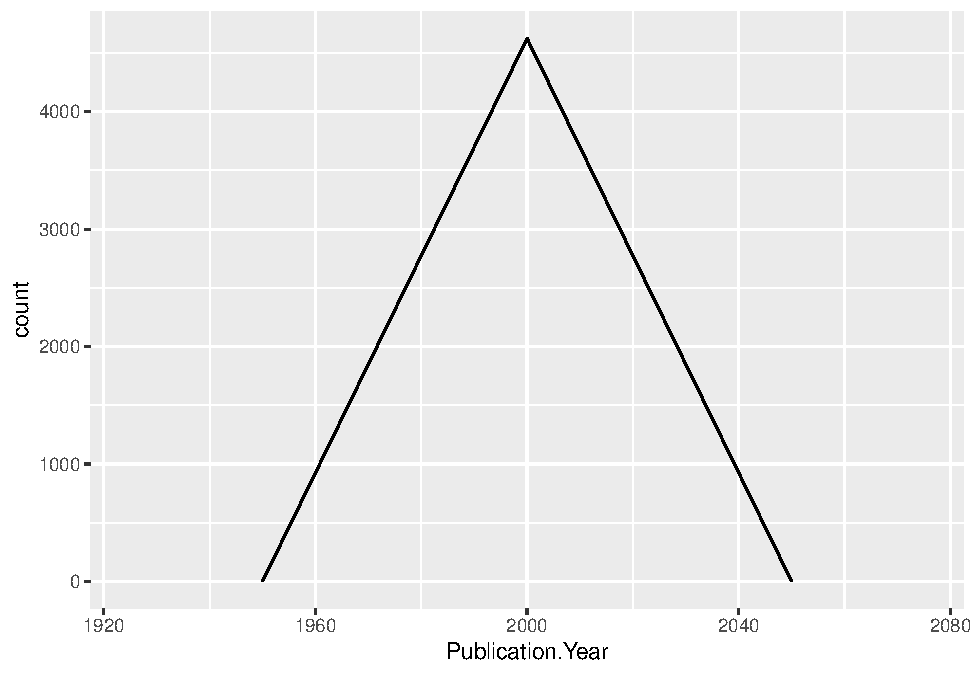
\includegraphics{A03_DataExploration_files/figure-latex/unnamed-chunk-6-1.pdf}

\begin{enumerate}
\def\labelenumi{\arabic{enumi}.}
\setcounter{enumi}{9}
\tightlist
\item
  Reproduce the same graph but now add a color aesthetic so that
  different Test.Location are displayed as different colors.
\end{enumerate}

\begin{Shaded}
\begin{Highlighting}[]
\KeywordTok{ggplot}\NormalTok{(Neonics) }\OperatorTok{+}
\StringTok{  }\KeywordTok{geom_freqpoly}\NormalTok{(}\KeywordTok{aes}\NormalTok{(}\DataTypeTok{x =}\NormalTok{ Publication.Year, }\DataTypeTok{bins =} \DecValTok{50}\NormalTok{, }\DataTypeTok{color =}\NormalTok{ Test.Location))}
\end{Highlighting}
\end{Shaded}

\begin{verbatim}
## Warning: Ignoring unknown aesthetics: bins
\end{verbatim}

\begin{verbatim}
## `stat_bin()` using `bins = 30`. Pick better value with `binwidth`.
\end{verbatim}

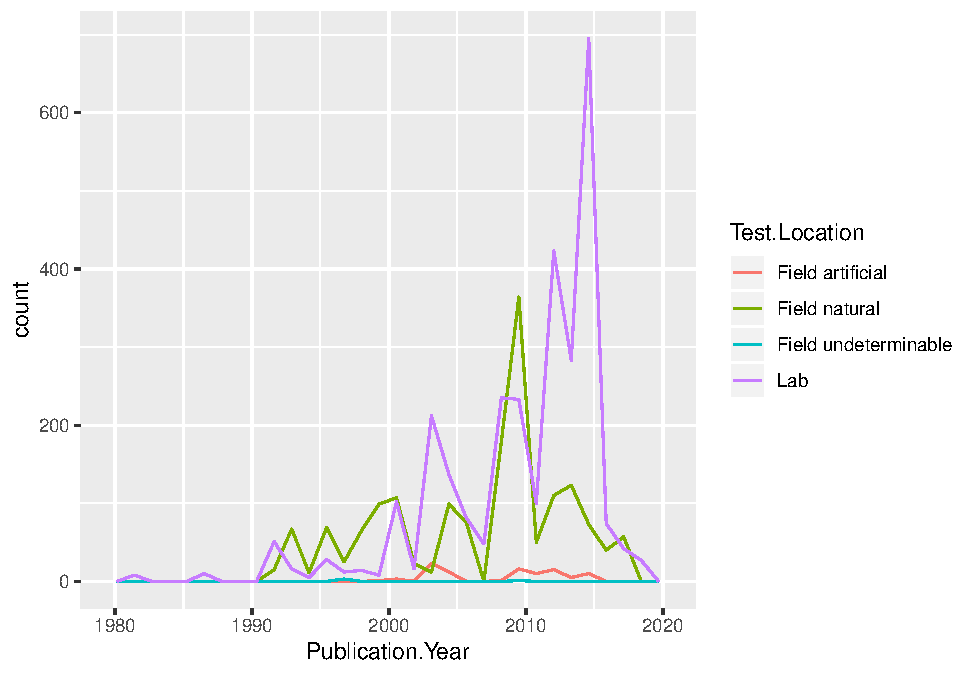
\includegraphics{A03_DataExploration_files/figure-latex/unnamed-chunk-7-1.pdf}

Interpret this graph. What are the most common test locations, and do
they differ over time?

\section{\textgreater{} Answer: The most common test locations are Lab
and Field natural. Both of these test locations differ over time as the
count is fewer in the 1990s and early 2000s and grows significantly from
\textasciitilde{}2008 to 2015. Both counts drop after
2015.}\label{answer-the-most-common-test-locations-are-lab-and-field-natural.-both-of-these-test-locations-differ-over-time-as-the-count-is-fewer-in-the-1990s-and-early-2000s-and-grows-significantly-from-2008-to-2015.-both-counts-drop-after-2015.}

\begin{enumerate}
\def\labelenumi{\arabic{enumi}.}
\setcounter{enumi}{10}
\tightlist
\item
  Create a bar graph of Endpoint counts. What are the two most common
  end points, and how are they defined? Consult the ECOTOX\_CodeAppendix
  for more information.
\end{enumerate}

\begin{Shaded}
\begin{Highlighting}[]
\NormalTok{NeonicsBargraph <-}\StringTok{ }\KeywordTok{ggplot}\NormalTok{(Neonics, }\KeywordTok{aes}\NormalTok{(}\DataTypeTok{x =}\NormalTok{ Endpoint)) }\OperatorTok{+}
\StringTok{  }\KeywordTok{geom_bar}\NormalTok{()}

\NormalTok{NeonicsBargraph}
\end{Highlighting}
\end{Shaded}

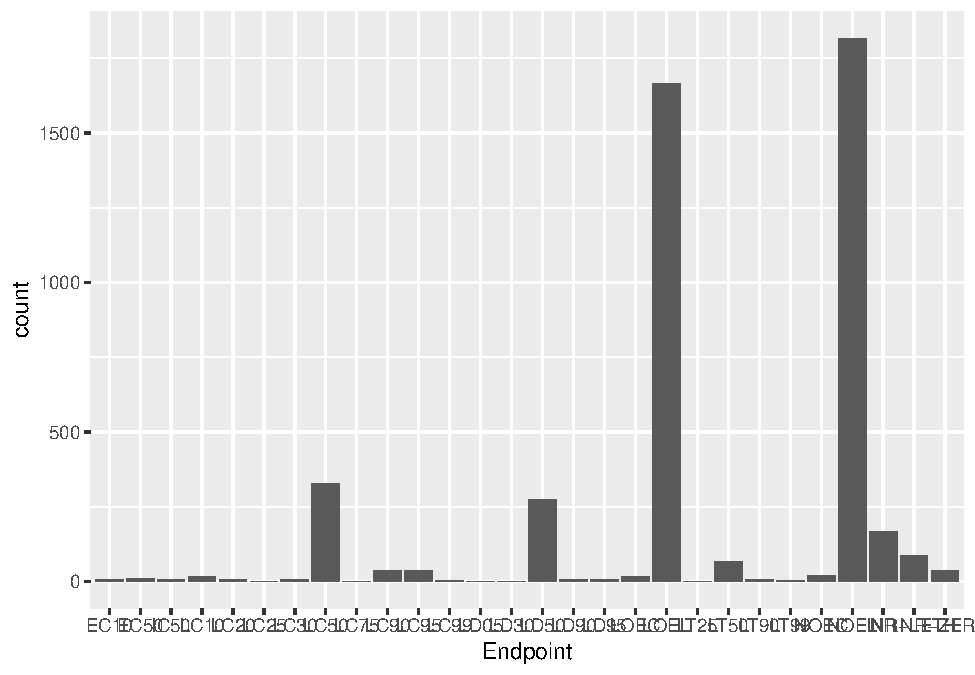
\includegraphics{A03_DataExploration_files/figure-latex/unnamed-chunk-8-1.pdf}

\section{\textgreater{} Answer: LOEL and NOEL and the two most common
end points. LOEL means Lowest-observable-effect-level and is defined as
the lowest dose (concentration) producing effects that were
significantly different from responses of controls. NOEL means
No-observable-effect-level and is defined as the highest dose
(concentration) producing effects not significantly different from
responses of controls according to author's reported statistical
test.}\label{answer-loel-and-noel-and-the-two-most-common-end-points.-loel-means-lowest-observable-effect-level-and-is-defined-as-the-lowest-dose-concentration-producing-effects-that-were-significantly-different-from-responses-of-controls.-noel-means-no-observable-effect-level-and-is-defined-as-the-highest-dose-concentration-producing-effects-not-significantly-different-from-responses-of-controls-according-to-authors-reported-statistical-test.}

\subsection{Explore your data (Litter)}\label{explore-your-data-litter}

\begin{enumerate}
\def\labelenumi{\arabic{enumi}.}
\setcounter{enumi}{11}
\tightlist
\item
  Determine the class of collectDate. Is it a date? If not, change to a
  date and confirm the new class of the variable. Using the
  \texttt{unique} function, determine which dates litter was sampled in
  August 2018.
\end{enumerate}

\begin{Shaded}
\begin{Highlighting}[]
\KeywordTok{view}\NormalTok{(Litter)}

\KeywordTok{class}\NormalTok{(Litter}\OperatorTok{$}\NormalTok{collectDate)}
\end{Highlighting}
\end{Shaded}

\begin{verbatim}
## [1] "factor"
\end{verbatim}

\begin{Shaded}
\begin{Highlighting}[]
\NormalTok{Litter}\OperatorTok{$}\NormalTok{collectDate <-}\StringTok{ }\KeywordTok{as.Date}\NormalTok{(Litter}\OperatorTok{$}\NormalTok{collectDate)}

\NormalTok{Litter}\OperatorTok{$}\NormalTok{collectDate}
\end{Highlighting}
\end{Shaded}

\begin{verbatim}
##   [1] "2018-08-02" "2018-08-02" "2018-08-02" "2018-08-02" "2018-08-02"
##   [6] "2018-08-02" "2018-08-02" "2018-08-02" "2018-08-02" "2018-08-02"
##  [11] "2018-08-02" "2018-08-02" "2018-08-02" "2018-08-02" "2018-08-02"
##  [16] "2018-08-02" "2018-08-02" "2018-08-02" "2018-08-02" "2018-08-02"
##  [21] "2018-08-02" "2018-08-02" "2018-08-02" "2018-08-02" "2018-08-02"
##  [26] "2018-08-02" "2018-08-02" "2018-08-02" "2018-08-02" "2018-08-02"
##  [31] "2018-08-02" "2018-08-02" "2018-08-02" "2018-08-02" "2018-08-02"
##  [36] "2018-08-02" "2018-08-02" "2018-08-02" "2018-08-02" "2018-08-02"
##  [41] "2018-08-02" "2018-08-02" "2018-08-02" "2018-08-02" "2018-08-02"
##  [46] "2018-08-02" "2018-08-02" "2018-08-02" "2018-08-02" "2018-08-02"
##  [51] "2018-08-02" "2018-08-02" "2018-08-02" "2018-08-02" "2018-08-02"
##  [56] "2018-08-02" "2018-08-02" "2018-08-02" "2018-08-02" "2018-08-02"
##  [61] "2018-08-02" "2018-08-02" "2018-08-02" "2018-08-02" "2018-08-02"
##  [66] "2018-08-02" "2018-08-02" "2018-08-02" "2018-08-02" "2018-08-02"
##  [71] "2018-08-02" "2018-08-02" "2018-08-02" "2018-08-02" "2018-08-02"
##  [76] "2018-08-02" "2018-08-02" "2018-08-02" "2018-08-02" "2018-08-02"
##  [81] "2018-08-02" "2018-08-02" "2018-08-02" "2018-08-02" "2018-08-02"
##  [86] "2018-08-02" "2018-08-02" "2018-08-02" "2018-08-02" "2018-08-02"
##  [91] "2018-08-02" "2018-08-30" "2018-08-30" "2018-08-30" "2018-08-30"
##  [96] "2018-08-30" "2018-08-30" "2018-08-30" "2018-08-30" "2018-08-30"
## [101] "2018-08-30" "2018-08-30" "2018-08-30" "2018-08-30" "2018-08-30"
## [106] "2018-08-30" "2018-08-30" "2018-08-30" "2018-08-30" "2018-08-30"
## [111] "2018-08-30" "2018-08-30" "2018-08-30" "2018-08-30" "2018-08-30"
## [116] "2018-08-30" "2018-08-30" "2018-08-30" "2018-08-30" "2018-08-30"
## [121] "2018-08-30" "2018-08-30" "2018-08-30" "2018-08-30" "2018-08-30"
## [126] "2018-08-30" "2018-08-30" "2018-08-30" "2018-08-30" "2018-08-30"
## [131] "2018-08-30" "2018-08-30" "2018-08-30" "2018-08-30" "2018-08-30"
## [136] "2018-08-30" "2018-08-30" "2018-08-30" "2018-08-30" "2018-08-30"
## [141] "2018-08-30" "2018-08-30" "2018-08-30" "2018-08-30" "2018-08-30"
## [146] "2018-08-30" "2018-08-30" "2018-08-30" "2018-08-30" "2018-08-30"
## [151] "2018-08-30" "2018-08-30" "2018-08-30" "2018-08-30" "2018-08-30"
## [156] "2018-08-30" "2018-08-30" "2018-08-30" "2018-08-30" "2018-08-30"
## [161] "2018-08-30" "2018-08-30" "2018-08-30" "2018-08-30" "2018-08-30"
## [166] "2018-08-30" "2018-08-30" "2018-08-30" "2018-08-30" "2018-08-30"
## [171] "2018-08-30" "2018-08-30" "2018-08-30" "2018-08-30" "2018-08-30"
## [176] "2018-08-30" "2018-08-30" "2018-08-30" "2018-08-30" "2018-08-30"
## [181] "2018-08-30" "2018-08-30" "2018-08-30" "2018-08-30" "2018-08-30"
## [186] "2018-08-30" "2018-08-30" "2018-08-30"
\end{verbatim}

\begin{Shaded}
\begin{Highlighting}[]
\KeywordTok{class}\NormalTok{(Litter}\OperatorTok{$}\NormalTok{collectDate)}
\end{Highlighting}
\end{Shaded}

\begin{verbatim}
## [1] "Date"
\end{verbatim}

\begin{Shaded}
\begin{Highlighting}[]
\KeywordTok{unique}\NormalTok{(Litter[,}\StringTok{"collectDate"}\NormalTok{])}
\end{Highlighting}
\end{Shaded}

\begin{verbatim}
## [1] "2018-08-02" "2018-08-30"
\end{verbatim}

\begin{enumerate}
\def\labelenumi{\arabic{enumi}.}
\setcounter{enumi}{12}
\tightlist
\item
  Using the \texttt{unique} function, determine how many plots were
  sampled at Niwot Ridge. How is the information obtained from
  \texttt{unique} different from that obtained from \texttt{summary}?
\end{enumerate}

\begin{Shaded}
\begin{Highlighting}[]
\KeywordTok{summary}\NormalTok{(Litter}\OperatorTok{$}\NormalTok{plotID)}
\end{Highlighting}
\end{Shaded}

\begin{verbatim}
## NIWO_040 NIWO_041 NIWO_046 NIWO_047 NIWO_051 NIWO_057 NIWO_058 NIWO_061 
##       20       19       18       15       14        8       16       17 
## NIWO_062 NIWO_063 NIWO_064 NIWO_067 
##       14       14       16       17
\end{verbatim}

\begin{Shaded}
\begin{Highlighting}[]
\KeywordTok{unique}\NormalTok{(Litter[}\StringTok{"plotID"}\NormalTok{])}
\end{Highlighting}
\end{Shaded}

\begin{verbatim}
##       plotID
## 1   NIWO_061
## 9   NIWO_064
## 17  NIWO_067
## 25  NIWO_040
## 35  NIWO_041
## 37  NIWO_063
## 48  NIWO_047
## 56  NIWO_051
## 63  NIWO_058
## 74  NIWO_046
## 84  NIWO_062
## 163 NIWO_057
\end{verbatim}

\begin{quote}
Answer: The `unique' function eliminates duplicate elements from the
column whereas the `summary' function produces result summaries of the
number of times each Plot ID is present.
\end{quote}

\begin{enumerate}
\def\labelenumi{\arabic{enumi}.}
\setcounter{enumi}{13}
\tightlist
\item
  Create a bar graph of functionalGroup counts. This shows you what type
  of litter is collected at the Niwot Ridge sites. Notice that litter
  types are fairly equally distributed across the Niwot Ridge sites.
\end{enumerate}

\begin{Shaded}
\begin{Highlighting}[]
\NormalTok{LitterBargraph <-}\StringTok{ }\KeywordTok{ggplot}\NormalTok{(Litter, }\KeywordTok{aes}\NormalTok{(}\DataTypeTok{x =}\NormalTok{ functionalGroup)) }\OperatorTok{+}
\StringTok{  }\KeywordTok{geom_bar}\NormalTok{()}

\NormalTok{LitterBargraph}
\end{Highlighting}
\end{Shaded}

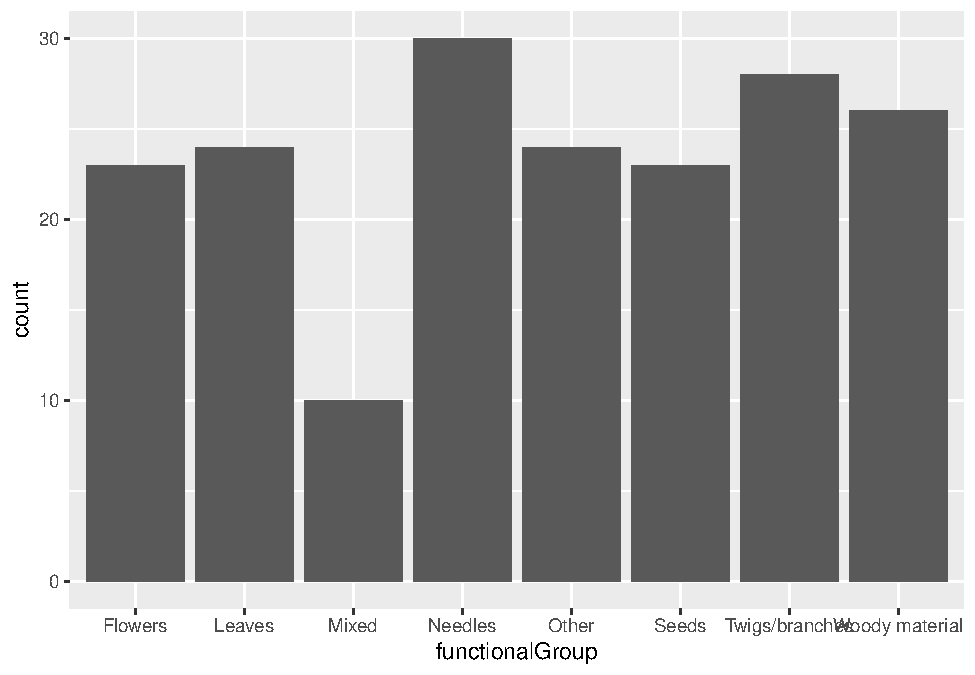
\includegraphics{A03_DataExploration_files/figure-latex/unnamed-chunk-11-1.pdf}

\begin{enumerate}
\def\labelenumi{\arabic{enumi}.}
\setcounter{enumi}{14}
\tightlist
\item
  Using \texttt{geom\_boxplot} and \texttt{geom\_violin}, create a
  boxplot and a violin plot of dryMass by functionalGroup.
\end{enumerate}

\begin{Shaded}
\begin{Highlighting}[]
\CommentTok{# Box Plot}

\KeywordTok{ggplot}\NormalTok{(Litter) }\OperatorTok{+}
\StringTok{  }\KeywordTok{geom_boxplot}\NormalTok{(}\KeywordTok{aes}\NormalTok{(}\DataTypeTok{x =}\NormalTok{ functionalGroup, }\DataTypeTok{y =}\NormalTok{ dryMass, }\DataTypeTok{group =} \KeywordTok{cut_width}\NormalTok{(functionalGroup, }\DecValTok{1}\NormalTok{)))}
\end{Highlighting}
\end{Shaded}

\includegraphics{A03_DataExploration_files/figure-latex/unnamed-chunk-12-1.pdf}

\begin{Shaded}
\begin{Highlighting}[]
\CommentTok{# Violin Plot}

\KeywordTok{ggplot}\NormalTok{(Litter) }\OperatorTok{+}
\StringTok{  }\KeywordTok{geom_violin}\NormalTok{(}\KeywordTok{aes}\NormalTok{(}\DataTypeTok{x =}\NormalTok{ functionalGroup, }\DataTypeTok{y =}\NormalTok{ dryMass),}
              \DataTypeTok{draw_quantiles =} \KeywordTok{c}\NormalTok{(}\FloatTok{0.25}\NormalTok{, }\FloatTok{0.5}\NormalTok{, }\FloatTok{0.75}\NormalTok{), }
              \DataTypeTok{scale =} \StringTok{"count"}\NormalTok{)}
\end{Highlighting}
\end{Shaded}

\begin{verbatim}
## Warning in regularize.values(x, y, ties, missing(ties)): collapsing to unique
## 'x' values

## Warning in regularize.values(x, y, ties, missing(ties)): collapsing to unique
## 'x' values

## Warning in regularize.values(x, y, ties, missing(ties)): collapsing to unique
## 'x' values
\end{verbatim}

\includegraphics{A03_DataExploration_files/figure-latex/unnamed-chunk-12-2.pdf}

Why is the boxplot a more effective visualization option than the violin
plot in this case?

\section{\textgreater{} Answer: The boxplot is more effective in this
case because it allows you to see the middle 50\% of the data
distribution and any outliers. The violin plot doesn't tell you much
because there there are many more counts of dryMass than functionalGroup
so you can't really tell what the plot is
signifying.}\label{answer-the-boxplot-is-more-effective-in-this-case-because-it-allows-you-to-see-the-middle-50-of-the-data-distribution-and-any-outliers.-the-violin-plot-doesnt-tell-you-much-because-there-there-are-many-more-counts-of-drymass-than-functionalgroup-so-you-cant-really-tell-what-the-plot-is-signifying.}

What type(s) of litter tend to have the highest biomass at these sites?

\section{\textgreater{} Answer: Needles tend to have the highest biomass
at these
sites.}\label{answer-needles-tend-to-have-the-highest-biomass-at-these-sites.}

\end{document}
